\section*{Assignment 01: Platform Concept and Value Proposition}
\addcontentsline{toc}{section}{Assignment 01: Platform Concept and Value Proposition}

SkillSync is my attempt to operationalise what \citet{Choudary2016} calls an "interaction first" platform. The two participant sets are students who crave scoped practice and civic organisations that need structured help but cannot afford consultants. Following \citet{Choudary2016}, I focus on three building blocks: a well defined value unit, clear producers and consumers, and repeatable matching rules. The value unit here is a time boxed project brief plus a student response. Students act as producers because they package skills, while organisations consume the value by commissioning projects. Matching rules rely on institutional email verification, a scoping checklist, and reputation scores so that quality stays legible before either side commits \citep{Lecture02}.

The idea crystallised only after testing alternative concepts against theory. A first draft imagined a dinner party marketplace, yet \citet{Srnicek2017} warns that platforms drift toward service businesses when they control assets, and that is exactly what the dinner idea required. Replaying Lecture~2 with those notes on my desk pushed me toward a design where the platform stays an orchestrator instead of becoming a logistics company. I sketched SkillSync again using \citet{Choudary2016}'s participation formula (access, ability, incentive). Access is guaranteed through campus logins and NGO invitations, ability is supported via templates and mentor nudges, and incentives include public endorsements plus optional stipends. Iterating through the formula made me spell out the mechanics rather than rely on hype.

Data loops keep the promise coherent. Every completed project would collect structured feedback on delivery, collaboration, and impact. Those signals feed matching weights, update a living skill taxonomy, and unlock richer badges for students so the system compounds value over time \citep{Lecture05}. On the organisation side the same data populates case studies and benchmark dashboards, keeping them motivated to return. \citet{Zuboff2019} reminds us to treat data as power, so the plan pairs analytics with explicit consent flows and opt in sharing that appear in Assignment~05.

Figure~\ref{fig:student-view} illustrates the application workspace a student opens when an organisation publishes a brief. The left column lists purpose, stipend range, estimated effort, and required outcomes with the copywriting pulled from the scoping checklist. The right column keeps the call to action, contact details, and timeline alerts visible. That layout deliberately reflects \citet{Choudary2016}'s interaction design advice: eliminate uncertainty around the core exchange and surface trust signals during decision moments.

\begin{figure}[H]
  \centering
  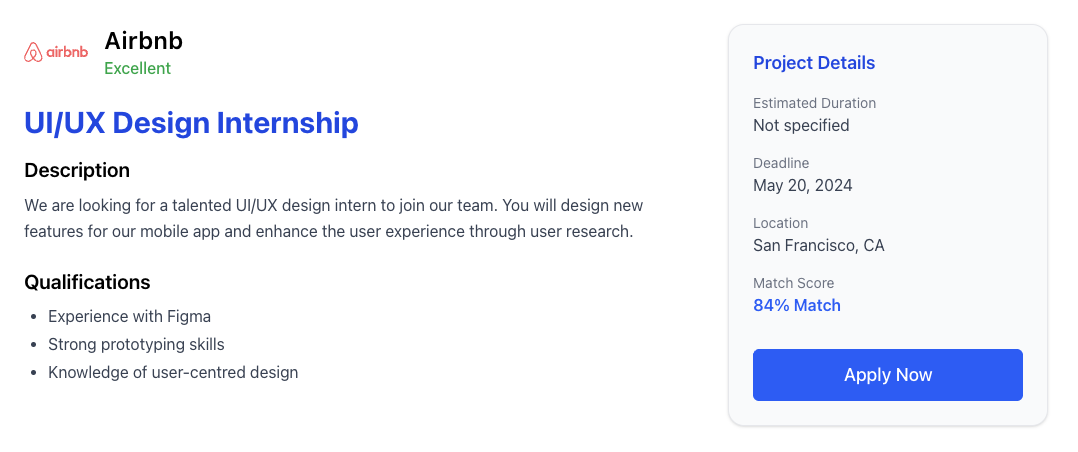
\includegraphics[width=0.85\linewidth]{figures/Student-Project-View.png}
  \caption{Student project workspace mock up with progress nudges.}
  \label{fig:student-view}
\end{figure}

The organisational journey mirrors the same interaction template. Their wizard requests outcome, support promises, success metrics, and timeline before anything goes live. That structure borrows explicitly from \citet{Reillier2017}'s recommendation to choreograph value creation steps and embed governance into the flow. Desk interviews from the course showed NGOs losing trust when briefs start vague, so the scoping wizard and student workspace were drafted together as a single interaction loop rather than separate screens.
